% Full body of the Q2/Q3 paper; intended for deliberate later integration.
% Includes its own title, symbols, references, and appendices.
\begin{center}
{\LARGE\bfseries 全向干扰源的主动定位与状态搜索}\\[7pt]
{\large 第二问与第三问论文稿}
\end{center}
\vspace{4pt}
\section{符号说明}\label{ux7b26ux53f7ux8bf4ux660e}

本文针对全向干扰源，将第二问的主动检测点选择作为第三问多源搜索的局部模块。先建立可保证接收和可靠清除的几何条件，再研究覆盖任务、已知源处理及测量费用的联合调度。下文的源位置可行域由观测构造，所有实验表中的用时均为题目动作计费时间，程序计算耗时单独说明。

\Needspace{38mm}
\begin{center}\small 表1 主要符号与含义\end{center}
\nopagebreak
\begin{longtable}[]{@{}
  >{\raggedright\arraybackslash}p{(\linewidth - 6\tabcolsep) * \real{0.2500}}
  >{\raggedright\arraybackslash}p{(\linewidth - 6\tabcolsep) * \real{0.2500}}
  >{\raggedright\arraybackslash}p{(\linewidth - 6\tabcolsep) * \real{0.2500}}
  >{\raggedright\arraybackslash}p{(\linewidth - 6\tabcolsep) * \real{0.2500}}@{}}

\toprule\noalign{}
\begin{minipage}[b]{\linewidth}\raggedright
符号
\end{minipage} & \begin{minipage}[b]{\linewidth}\raggedright
含义
\end{minipage} & \begin{minipage}[b]{\linewidth}\raggedright
符号
\end{minipage} & \begin{minipage}[b]{\linewidth}\raggedright
含义
\end{minipage} \\
\midrule\noalign{}
\endfirsthead
\toprule\noalign{}
\begin{minipage}[b]{\linewidth}\raggedright
符号
\end{minipage} & \begin{minipage}[b]{\linewidth}\raggedright
含义
\end{minipage} & \begin{minipage}[b]{\linewidth}\raggedright
符号
\end{minipage} & \begin{minipage}[b]{\linewidth}\raggedright
含义
\end{minipage} \\
\midrule\noalign{}
\endhead
\bottomrule\noalign{}
\endlastfoot
\(\Omega\) & 半径1800 m目标圆域 & \(f\) & 测向频道，1至20 \\
\(p\) & 源坐标 & \(x_t\) & 当前机器人位置 \\
\(R_f\) & 固定但未知的接收半径 & \(\bar\varepsilon\) & 含舍入余量的测角误差界 \\
\(\widehat C_f\) & 源位置的凸外包区域 & \(Q_f\) & 保证再次接收的测点域 \\
\(z(C),\rho(C)\) & 最小包围圆的圆心与半径 & \(v\) & 移速，5 m/s \\
\(\mathcal D_t,\mathcal K_t\) & 已发现及已清除频道集合 & \(M,j\) & 任务位掩码与最后任务 \\
\(L,T\) & 实际路长与计费用时 & \(U_t,L_t\) & 冻结规划问题的上界与下界 \\
\end{longtable}

\section{问题二　保证接收条件下的主动交会定位}\label{ux95eeux9898ux4e8c-ux4fddux8bc1ux63a5ux6536ux6761ux4ef6ux4e0bux7684ux4e3bux52a8ux4ea4ux4f1aux5b9aux4f4d}

一次示向度只能确定干扰源所在的狭长角域，沿示向方向移动虽然能够接近部分可能位置，却未必明显改善交会精度。第二检测点的选择需要同时回答两个问题：到达该点后能否再次接收到信号，以及新增观测能否以较小移动代价缩小定位区域。为此，先由首测信息构造保证接收的候选域，再在其中选择兼顾接近距离与残余不确定性的检测点。本节建立的单源模块将在第三问中反复调用。

\subsection{2.1 首次观测与源位置可行域}\label{ux9996ux6b21ux89c2ux6d4bux4e0eux6e90ux4f4dux7f6eux53efux884cux57df}

记频道 \(f\) 的源坐标为 \(p\)，首个检测点为 \(x_1\)，测得示向度为 \(\theta_1\)；目标区域为 \(\Omega=\{p:\|p\|\le1800\}\)。接收半径 \(R_f\) 在单次测试中固定，但其数值未知，满足 \(R_{\min}=1000\le R_f\le R_{\max}=1500\)。题面给出的测角误差界为 \(\varepsilon=1^\circ\)。程序读取两位小数的角度时采用 \(\bar\varepsilon=1.005^\circ\)，额外的 \(0.005^\circ\) 用于保守容纳角度舍入，并非改变题设误差范围。

令 \(u(\alpha)=(\cos\alpha,\sin\alpha)\)，首测对应的前向角域为

\[
W(x_1,\theta_1)=\left\{p:
u(\theta_1-\bar\varepsilon)\times(p-x_1)\ge0,\quad
u(\theta_1+\bar\varepsilon)\times(p-x_1)\le0
\right\}.
\tag{2-1}
\]

因此可保守保留

\[
C_f^{(1)}=\Omega\cap B(x_1,R_{\max})\cap W(x_1,\theta_1).
\tag{2-2}
\]

其中 \(B(x,r)\) 表示闭圆盘。获得示向度还意味着距离大于 \(5\) m；省略这一个内圆排除能够保持凸性，只会扩大候选集。实现时将两个圆约束换成外切正128边形，得到包含 \(C_f^{(1)}\) 的凸多边形 \(\widehat C_f^{(1)}\)。以下选点与清除均依据该外包多边形，避免离散近似误删合法位置。记 \(\rho(C)=\min_z\max_{p\in C}\|p-z\|\)，并以 \(z(C)\) 表示最小包围圆圆心。

\subsection{2.2 保证再次接收的第二点候选域}\label{ux4fddux8bc1ux518dux6b21ux63a5ux6536ux7684ux7b2cux4e8cux70b9ux5019ux9009ux57df}

第二次检测若失去信号，便无法直接形成双站交会。利用全向源的最小接收半径，定义

\[
Q_f=\bigcap_{p\in\widehat C_f^{(1)}}B(p,R_{\min})
=\left\{x:\max_{p\in\widehat C_f^{(1)}}\|x-p\|\le1000\right\}.
\tag{2-3}
\]

对任意 \(x\in Q_f\)，真实源必有 \(\|x-p\|\le1000\le R_f\)，因而必然返回示向度或近场反馈。若外包多边形顶点集合为 \(V_f\)，则

\[
Q_f=\bigcap_{a\in V_f}B(a,1000).
\tag{2-4}
\]

证明只需利用凸性：任意 \(p=\sum_a\lambda_a a\) 满足 \(\|x-p\|\le\sum_a\lambda_a\|x-a\|\)。所以检查全部顶点即能核验候选点，无须枚举区域内部。

该候选域并不要求预先知道源的距离。外切128边形的最远顶点距离不超过 \(\widetilde R=R_{\max}\sec(\pi/128)\)，故忽略目标圆截断后，外包区域仍位于长度 \(\widetilde R\)、半角 \(\bar\varepsilon\) 的扇形内。该扇形可被下列圆覆盖：

\[
z_0=x_1+\frac{\widetilde R}{2\cos\bar\varepsilon}u(\theta_1),
\qquad r_0=\frac{\widetilde R}{2\cos\bar\varepsilon}<1000.
\tag{2-5}
\]

这是因为沿任一射线的距离平方关于径向坐标为凸函数，其最大值在径向两端取得，代入即可验证。故 \(B(z_0,1000-r_0)\subseteq Q_f\) 是一个明确的安全候选子域；考虑目标圆截断后，源的不确定性只会减小。程序仍通过式(2-4)逐点重新核验候选位置。

式(2-3)给出容易计算的充分候选域，并非最大的保证接收域。首测已接收还隐含 \(R_f\ge\|p-x_1\|\)，若联合保留源位置与接收半径，可进一步放宽部分检测点限制。本方法使用统一的1000 m保证，以便在后续多次观测中直接复用。

\subsection{2.3 依据区域长轴构造有限探点}\label{ux4f9dux636eux533aux57dfux957fux8f74ux6784ux9020ux6709ux9650ux63a2ux70b9}

交会定位的一阶误差随两条视线夹角的正弦减小而放大。因此，候选点既应包含沿首测方向接近区域的点，也应包含能够产生横向基线的点。令 \(z=z(\widehat C_f)\)，当前位置为 \(x_0\)，首测方向的单位法向量为 \(n_1=(-\sin\theta_1,\cos\theta_1)\)。先构造9个基础点：

\[
A_0=\{z\}\cup\left\{
x_0+t(z-x_0)+b n_1:
t\in\{1/2,1\},\ b\in\{-150,-50,50,150\}
\right\}.
\tag{2-6}
\]

再取多边形最远顶点对的方向为单位长轴 \(e\)，其法向量为 \(e_\perp\)。将所有顶点相对 \(z\) 投影到长轴，得到区间 \([\ell_-,\ell_+]\)，令 \(w=\ell_+-\ell_-\)、\(b_*=\min\{200,\max\{20,w/8\}\}\)。补充

\[
\begin{aligned}
A_1={}&\{z+(\ell_-+tw)e+b e_\perp:
t\in\{1/4,3/8,5/8,3/4\},\ b\in\{-b_*,0,b_*\}\}\\
&\cup\{z-b_*e_\perp,z+b_*e_\perp\}.
\end{aligned}
\tag{2-7}
\]

实现先在 \(A_0\) 中寻找满足式(2-4)的有效新点；存在基础候选时，再扩展至 \(A_0\cup A_1\)。删除重复点、同频道已测位置和不满足保证接收条件的点后，候选总数至多23个。内侧的 \(3/8\)、\(5/8\) 位置有助于在首测角域较长、外侧探点难以保证接收时保留横向选择。第二问中 \(x_0=x_1\)；第三问则以当前实时位置和更新区域调用这一子程序。后续多次定位若基础集合中已无合法新点，先尝试包围圆心及其180 m以内偏移点，再无新点则执行有限光学网格。由于后续区域只收缩，式(2-5)保证其包围圆半径小于751 m，偏移回退点到任一可能源的距离小于 \(751+180<1000\) m，仍保持接收保证；这一证明依赖区域更新正确且区域非空。

\subsection{2.4 有限名义观测下的选点评分}\label{ux6709ux9650ux540dux4e49ux89c2ux6d4bux4e0bux7684ux9009ux70b9ux8bc4ux5206}

仅按移动距离选点可能保留过长的定位区域，仅追求区域最小又可能付出过大的绕行代价。为同时反映这两方面，从当前区域选取至多5个名义源点：包围圆心 \(z\)，以及至多4个均匀抽取顶点沿连线向圆心移动四分之一所得的位置。该集合记为 \(H_f=\{p^{(1)},\ldots,p^{(h)}\}\)，仅用于有限几何评价。

对于候选点 \(x\) 和名义源点 \(p^{(k)}\)，若二者距离大于5 m，则计算无附加误差的名义示向度，在区域副本中增加一次角度约束，得到残余半径 \(r_k(x)\)。若距离不超过5 m，则按近场反馈处理。取移动速度 \(v=5\) m/s、可靠清除门限 \(r_c=19.9\) m，定义

\[
\begin{aligned}
J(x)&=\frac{\|x-x_0\|}{v}
+\frac1h\sum_{k=1}^{h}\left[\frac{\|x-p^{(k)}\|}{v}+P_k(x)\right],\\
P_k(x)&=\begin{cases}
0,&\|x-p^{(k)}\|\le5,\\
6\,\mathbf1_{\{r_k(x)>r_c\}}
+\kappa\dfrac{(r_k(x)-r_c)_+}{v},&\text{其他情形},
\end{cases}\qquad\kappa=0.5.
\end{aligned}
\tag{2-8}
\]

其中前两项衡量到探点及从探点接近名义源的移动代价；6 s罚项近似反映仍需一次测量和换频的代价；超出清除尺度的半径罚项抑制信息不足的探点。对固定频道，当前检测及换频费用对所有候选相同，故不影响排序。选择 \(J\) 最小的候选，并按横、纵坐标依次打破平局。计算时先用不含非负罚项的部分建立下界，无法优于当前最优候选时提前停止该点评价。

等权名义点不代表已知的真实源后验分布，式(2-8)是有限代理目标，也不是所有误差下的最坏残余半径。因此，本节得到的是可执行的主动选点策略；有限候选的最小分值不等于连续候选域的全局最优。执行第二次检测后，只用真实反馈更新 \(\widehat C_f\)，再计算实际残余半径。若得到近场反馈，可在原位置清除；否则，是否达到20 m清除要求须由更新区域重新判定。

\par\noindent\begin{minipage}{\linewidth}
\textbf{算法1：单源主动检测点选择}

\begin{verbatim}
输入：当前点 x0、首测方向 θ1、源外包区域 Ĉf、同频道历史测点
1. 求 Ĉf 的包围圆心及长轴，先生成基础集合 A0。
2. 基础集合有有效新点时再扩展A1，去重并核验保证接收条件。
3. 构造名义源点集合 Hf；对每个 x 属于 A 计算式(2-8)。
4. 返回分值最小的 x；基础集合无新点时尝试圆心与偏移回退。
5. 执行真实测量，以真实反馈更新区域或触发近场清除。
\end{verbatim}
\end{minipage}\par


\begin{figure}[!htbp]
\centering
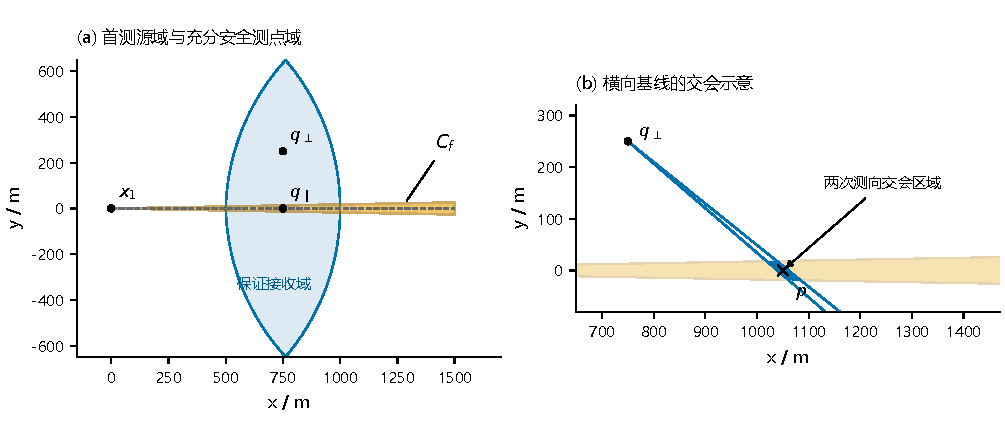
\includegraphics[width=\linewidth,height=\textheight,keepaspectratio,alt={图1 首测可行域及横向交会的解析示意。半角采用1.005°，蓝色测点域由三角外包构造，属于充分保证接收域；示意源p仅用于解释交会几何，不作为规划输入。右图展示另一比例下的局部几何，不能作为算法性能比较。}]{q23_figures/fig01_q2_geometry.pdf}
\caption{图1 首测可行域及横向交会的解析示意。半角采用1.005°，蓝色测点域由三角外包构造，属于充分保证接收域；示意源p仅用于解释交会几何，不作为规划输入。右图展示另一比例下的局部几何，不能作为算法性能比较。}
\end{figure}

\subsection{2.5 真实观测算例}\label{ux771fux5b9eux89c2ux6d4bux7b97ux4f8b}

在场景800035的状态搜索轨迹中，按动作发生时间选择首个``同频道第二次有效示向来自主动定位''的实例，得到频道 20。首测位于原点，第二测点由长轴分位候选策略实际选择；此前该频道没有负观测或推断约束，因此使用这两次示向即可重建当时的全部源区域信息。

\Needspace{38mm}
\begin{center}\small 表2 频道20的两次有效测量与区域收缩\end{center}
\nopagebreak
\begin{longtable}[]{@{}lcrr@{}}

\toprule\noalign{}
观测 & 检测点坐标 / m & 示向度 & 外包圆半径 / m \\
\midrule\noalign{}
\endfirsthead
\toprule\noalign{}
观测 & 检测点坐标 / m & 示向度 & 外包圆半径 / m \\
\midrule\noalign{}
\endhead
\bottomrule\noalign{}
\endlastfoot
原点首测 & (0.000, 0.000) & 125.00° & 750.226 \\
主动再测 & (-170.646, 568.027) & 148.14° & 65.012 \\
\end{longtable}

两检测点相距 593.106 m。第二点到首测外包区域各顶点的最大距离为 960.427 m，小于1000 m，满足保证再接收条件。第二次观测将外包最小包围圆半径由750.226 m缩小至65.012 m，降幅约 91.33\%，但尚未达到19.9 m可靠清除门限，因此仍需后续观测或光学覆盖。该例说明一次实际横向探测如何缩小可行域，不用于证明该选点优于所有其他候选。

重建沿用原评估版本的128边外切圆近似和1.005°计算半角；题面误差界仍为1°，额外0.005°用于舍入余量。算例仅由既有坐标和示向度重建，未使用真实源坐标选择实例；原始动作及重建数值见辅助材料。

以上构造同时给出了第二检测点的候选区域与可执行选择规则。其理论保证在于真实源保留、候选点可接收以及清除条件可靠；选点效率仍须由实际后续测量检验。本稿已有实验主要评估完整第三问，尚不把整局节省量当成第二检测点单独优越性的证据。

\section{问题三　基于状态压缩与覆盖约束的多源搜索}\label{ux95eeux9898ux4e09-ux57faux4e8eux72b6ux6001ux538bux7f29ux4e0eux8986ux76d6ux7ea6ux675fux7684ux591aux6e90ux641cux7d22}

第二问解决已发现单源的后续测点选择，第三问还需确定何时继续发现未知源、何时处理已知源，以及怎样确认任务完成。由于新观测不断改变可行域和任务集合，一次性规划所有真实源的最短路线并不可行。本文采用滚动规划：以合法观测维护源区域，将当前覆盖任务与定位清除任务合并为有限路线问题；每完成一个任务，再根据新信息重新规划。以下先给出状态搜索第一版的方法主体，再单列利用历史负观测的扫描精化，使不同版本的实验结果能够对应到明确算法。

\subsection{3.1 信息状态与总时间目标}\label{ux4fe1ux606fux72b6ux6001ux4e0eux603bux65f6ux95f4ux76eeux6807}

记第 \(t\) 次真实动作后的信息状态为

\[
S_t=\left(x_t,f_t,T_t,\mathcal D_t,\mathcal K_t,
\{\widehat C_f,\mathcal O_f^+,\mathcal O_f^-\},P_t,F_t\right).
\tag{3-1}
\]

其中 \(x_t,f_t\) 为位置和当前测向频道，\(T_t\) 为累计虚拟时间；\(\mathcal D_t\)、\(\mathcal K_t\) 分别记录已发现、已成功清除的频道；\(\mathcal O_f^+\)、\(\mathcal O_f^-\) 为同频道正、负反馈；\(P_t\) 为已完成的发现站集合，\(F_t\) 为未来覆盖站。源位置、实际源数和各源接收半径不进入决策状态。

总虚拟时间按实际动作计为

\[
T=\frac{L}{v}+N_{\rm switch}+5N_{\rm measure}
+3N_{\rm clear}+2K,\qquad v=5.
\tag{3-2}
\]

这里 \(N_{\rm clear}\) 包含成功与失败的光学尝试，\(K\) 为成功次数；清除不改变测向频道。优化目标是在全清约束下减小 \(T\)。算法自身的计算时间另外记录，不能与机器人虚拟时间混合。

正示向反馈按第二问更新区域。对于已确认存在的全向源，若在 \(x^+\) 有信号、在 \(x^-\) 无信号，由同一接收半径固定可得

\[
\|p-x^+\|\le R_f<\|p-x^-\|
\Longrightarrow
(x^--x^+)^Tp\le\frac{\|x^-\|^2-\|x^+\|^2}{2}.
\tag{3-3}
\]

右侧取闭半平面作为严格不等式的保守放宽。将新观测与所有异类历史观测配对裁剪，使无信号反馈也能够缩小区域。尚未出现正观测时只保存负点；不将一次无信号直接解释为频道无源。该距离关系依赖全向辐射，不能直接用于第四问。

\subsection{3.2 七点发现覆盖及覆盖点的连续调整}\label{ux4e03ux70b9ux53d1ux73b0ux8986ux76d6ux53caux8986ux76d6ux70b9ux7684ux8fdeux7eedux8c03ux6574}

先在原点扫描20个频道，再以原点与半径 \(a=1150\) m圆周上的6个等角站构成初始覆盖：

\[
P_0=\{(0,0)\}\cup
\{a(\cos(k\pi/3),\sin(k\pi/3)):k=0,\ldots,5\}.
\tag{3-4}
\]

对任意 \(p\in\Omega\)，若 \(\|p\|\le1000\)，则原点必能接收；否则记 \(r=\|p\|\in[1000,1800]\)，存在一个环上站与其极角相差不超过 \(30^\circ\)，于是

\[
\|p-x_k\|^2\le r^2+a^2-\sqrt3ar.
\tag{3-5}
\]

右侧关于 \(r\) 为凸函数，在该区间的最大值取于端点。代入 \(a=1150\)，两端均小于 \(1000^2\)，故七个站覆盖所有可能源位置。只要每个仍未知频道在覆盖站完成实际扫描，就不会遗漏全向源。已清除频道无须再测；已持有可靠清除位置的已知频道也可省略后续扫描。

固定覆盖站提供完整性，却可能迫使机器人在已知源附近绕行。因此允许移动一个尚未执行的站，同时保留全覆盖。设待改站为 \(x_i\)，\(G_i\) 包含已执行站与其余未来站，取 \(r_s=1000-10^{-5}\) m，尚需由此站负责的区域为

\[
E_i=\Omega\setminus\bigcup_{x\in G_i}B(x,r_s),
\qquad Q_i^{\rm cover}=\bigcap_{p\in E_i}B(p,r_s).
\tag{3-6}
\]

新站 \(y\in Q_i^{\rm cover}\) 即可保持覆盖；该集合是圆盘的交，因而为凸集。以旧站为起点，朝当前位置、邻近已知源代表点及相关投影点试探，沿线段二分寻找可行位置，再比较更新后的路线费用。每轮至多改变一个站，旧位置始终保留为可行备选。

实际覆盖核验计算

\[
\Gamma(P)=\max_{p\in\Omega}\min_{x\in P}\|p-x\|,
\tag{3-7}
\]

要求 \(\Gamma(P)\le r_s\)。计算检查最近站Voronoi结构的内部顶点、圆周交点与圆弧极值，不以只检查场地圆周代替全域覆盖。未来站的可行性属于计划约束；只有实际扫描完成后，才能计入发现证据。

\begin{figure}[!htbp]
\centering
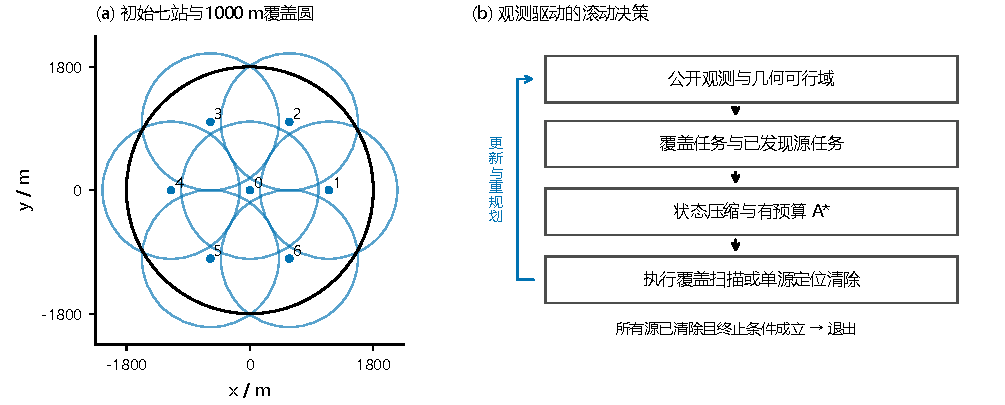
\includegraphics[width=\linewidth,height=\textheight,keepaspectratio,alt={图2 初始发现覆盖与滚动决策框架。七个1000 m接收保证圆覆盖半径1800 m场地；未来站移动后仍需重新通过全域覆盖核验。}]{q23_figures/fig02_framework.pdf}
\caption{图2 初始发现覆盖与滚动决策框架。七个1000 m接收保证圆覆盖半径1800 m场地；未来站移动后仍需重新通过全域覆盖核验。}
\end{figure}

\subsection{3.3 冻结任务的状态压缩与有预算A*搜索}\label{ux51bbux7ed3ux4efbux52a1ux7684ux72b6ux6001ux538bux7f29ux4e0eux6709ux9884ux7b97aux641cux7d22}

每完成一次覆盖扫描或一个源的处理，构造两类当前任务：尚未执行的覆盖站，以及已发现但未清除的源。源任务以近场点或可行域包围圆心作为代表位置 \(y_i\)。这些位置来自观测估计，实际定位仍由第二问模块完成，故源任务的代表点与最终清除点可以不同。

在本轮规划内冻结任务集合、位置和服务费用。设有 \(n\) 个任务，\(M\) 为已完成任务集合，程序以位掩码编码，\(j\) 为最后任务；起始状态 \((\varnothing,-1)\) 对应当前位置，约定 \(y_{-1}=x_t\)。借鉴子集动态规划{[}1{]}，将不同访问顺序压缩成相同的 \((M,j)\)，定义 \(g(M,j)\) 为到达该状态的最小前缀费用。转移为

\[
g(M\cup\{i\},i)=\min_j\left[g(M,j)+\Delta(M,j,i)\right],
\tag{3-8}
\]

\[
\Delta(M,j,i)=\frac{\|y_j-y_i\|}{v}+s_i
+q\,\mathbf1_{\{i\text{为覆盖任务}\}}\,|\mathcal S\setminus M|.
\tag{3-9}
\]

其中 \(\mathcal S\) 是本轮源任务集合，\(s_i\) 对源任务取5 s，对覆盖任务取 \(6b\) s，\(b=\max\{0,20-|\mathcal K_t|-|\mathcal S|\}\)。最后一项用于表示覆盖访问时尚未处理源的附加扫描费用。第一版选定配置取 \(q=0\)，使当前排序主要由旅行距离决定；实际测量与换频仍按式(3-2)完整计费。冻结服务费只用于比较候选路线，不替代实际时间账。

若两个前缀到达同一 \((M,j)\)，其后续任务、起点和费用函数完全相同，较贵前缀不会产生更优完整路线，因而可以删除。这一支配关系将排列枚举压缩为至多 \(O(n2^n)\) 个状态、\(O(n^22^n)\) 条转移。这里压缩的是一次规划中的任务顺序，并未把具有不同观测历史的真实世界状态强行合并。

采用A*启发式图搜索{[}2{]}，为优先探索有希望的前缀，对未完成任务集 \(U\) 构造下界

\[
h(M,j)=\frac{\min_{i\in U}\|y_j-y_i\|+\operatorname{MST}(U)}{v}
+\sum_{i\in U}s_i.
\tag{3-10}
\]

其中 \(U=\varnothing\) 时取零。任何完整后缀都必须先接入 \(U\)，再连通其中全部任务，其旅行距离不小于最近接入边加最小生成树；省略非负附加扫描费不会抬高下界。

算法先由最近邻和开路2-opt得到完整可行路线，费用记为 \(U_t\)；再按 \(g+h\) 从小到大展开，结合状态支配和 \(g+h\ge U_t\) 上界剪枝。发现更短完整路线时更新 \(U_t\)。预算耗尽则返回当前可行路线及前沿下界 \(L_t\)；搜索闭合时两界相等。实现保留 \(10^{-9}\) s比较容差，并允许改进状态重新入队。

当前任务至多22个；选定配置每次搜索至多展开100个状态，整局总展开上限为60000。只执行返回顺序的第一个任务，随后重新构造问题。\(U_t-L_t\) 衡量本轮冻结代理模型的求解缺口；未来新源、反馈分支和定位绕路未被完整枚举，因此它不是第三问在线最优策略的差距。

\subsection{3.4 主动定位、共享测量与可靠清除}\label{ux4e3bux52a8ux5b9aux4f4dux5171ux4eabux6d4bux91cfux4e0eux53efux9760ux6e05ux9664}

源任务执行时，先检查是否已有近场反馈或满足 \(\rho(\widehat C_f)\le r_c\)。若条件尚未满足，调用第二问的有限主动探点策略；每次得到真实反馈后重新计算区域，至多增加6次检测。

当包围圆为 \(B(z_f,r_f)\) 且 \(r_f\le r_c=19.9\) m时，所有满足

\[
x\in B(z_f,r_c-r_f)
\tag{3-11}
\]

的位置均可保证清除。因为对任意 \(p\in\widehat C_f\)，有 \(\|x-p\|\le\|x-z_f\|+r_f\le r_c<20\)。因此不必总走到圆心，可选择该安全圆中距当前位置最近的点；若当前位置已在圆内，则直接清除。

清除某个源后，当前位置还可能为其他已知源提供较好的交会基线。对保证接收且未测过的频道，若当前半径至少60 m，名义中心反馈预计使半径至少减半并减少30 m，则追加一次实际测量。该规则利用已经支付的移动成本；名义缩域仅决定是否测量，真实区域仍只由实际反馈及严格推断更新。

有限次主动测量未能达到清除尺度时，在候选区域上覆盖边长28 m的方格，并依次在所有相交单元中心执行光学清除。单元内任一点到中心的距离至多 \(28/\sqrt2<20\) m，故真实源所在单元必能被清除。区域有界，所需单元有限；这为局部任务提供有限兜底，但不要求每次光学尝试都成功。只有接口返回真实清除成功，才将该频道计入 \(\mathcal K_t\)。

\subsection{3.5 逻辑静默推断与扫描精化}\label{ux903bux8f91ux9759ux9ed8ux63a8ux65adux4e0eux626bux63cfux7cbeux5316}

已经发现的源在某个覆盖站必然无信号时，重复查询只会增加测量和换频费用。第一版使用接收半径上限：若

\[
\operatorname{dist}(x,\widehat C_f)>R_{\max},
\tag{3-12}
\]

则当前位置对所有可能源都超出接收距离，可省略该次物理检测，将结论作为推断负观测与已有正观测配对。实现增加 \(10^{-5}\) m裕量，且不为未知频道使用此项删测。

后续精化进一步利用同频道此前的真实负观测。设 \(n\) 为真实返回无信号的位置，拟检测点为 \(x\)。若 \(x\) 对当前区域中的每个可能源都比 \(n\) 更远，则由 \(\|p-n\|>R_f\) 可推出 \(\|p-x\|>R_f\)。展开平方差得到

\[
\|p-x\|^2-\|p-n\|^2
=2(n-x)^T\left(p-\frac{n+x}{2}\right).
\tag{3-13}
\]

这是关于 \(p\) 的仿射函数，最小值可在多边形顶点中求得。因此只需验证

\[
\min_{a\in V_f}(n-x)^T\left(a-\frac{n+x}{2}\right)>0.
\tag{3-14}
\]

这一条件可以覆盖式(3-12)尚不成立的部分位置。实现对加、减、乘结果采用向外浮点区间包络，要求保守下端点仍超过 \(10^{-5}\|n-x\|\) 的距离裕量；边界不确定时保留真实测量。这里的区间核验针对给定多边形顶点，源被多边形包含的前提仍依赖前述区域构造。

见证 \(n\) 必须来自同一未清除频道的历史真实动作，当前版本不使用推断点作为新的见证。推断不移动机器人、不切换频道，也不产生实际测量记录。对未知频道不能给予任何未经实际扫描的几何覆盖信用。

同一精化版本还在每个拟测频道前检查是否已发现16个不同源；一旦达到公开上限，后续未知频道可直接排除。已知但未清除的频道仍保留必要测量，所有已发现源仍须真实清除。这两项机制分别设置开关，便于通过消融区分各自作用。

\subsection{3.6 完整终止与算法流程}\label{ux5b8cux6574ux7ec8ux6b62ux4e0eux7b97ux6cd5ux6d41ux7a0b}

完整清除采用两种终止依据。第一种是16个不同频道均已真实清除，由源数上限立即确认完成。第二种是已执行站对所有仍未知频道形成完整发现覆盖，同时全部已发现源已清除且数量符合10---16的题设范围。仅清除当前发现的源不能推出全清；仅发现16个源也不能替代清除。

七点覆盖及逐站合法移动保证最终不会遗漏源，单源的有限光学网格保证能够结束局部清除。因此，在源静止、反馈符合规则、保守区域包含真值且时间与动作预算足够时，算法能够有限步完成任务。程序在每次动作前核查剩余预算；发生超时、反馈矛盾或未确认请求时保留未完成状态，不将中止当作成功。

\par\noindent\begin{minipage}{\linewidth}
\textbf{算法2：多源滚动搜索与清除}

\begin{verbatim}
输入：目标圆域 Ω、20个频道、源数范围10—16和设备动作费用
1. 从原点进入环境，扫描频道并初始化区域、已发现集与未来覆盖站。
2. 若已有16次不同频道的真实成功清除，确认完成并退出。
3. 构造剩余覆盖任务和已知源任务，冻结代表位置及代理服务费。
4. 用状态压缩A*求有限路线；允许一次经全域核验的未来站移动。
5. 若首任务为覆盖扫描：逐频道检查清除证书、静默证书和数量上限；
   对仍需查询的频道实际测量，只登记已完成的真实覆盖证据。
6. 若首任务为源处理：调用算法1，达到清除尺度即执行清除；
   有限探测不足时执行光学网格；完成后尝试有价值的共享测量。
7. 按实际反馈更新信息状态；检查完整覆盖及全部已知源清除条件。
8. 未完成且预算允许则返回步骤2；否则记录完成或中止原因并退出。
\end{verbatim}
\end{minipage}\par


\subsection{3.7 对照方法及学习模型}\label{ux5bf9ux7167ux65b9ux6cd5ux53caux5b66ux4e60ux6a21ux578b}

四类方法共同遵守设备反馈、几何清除和完整退出约束，区别在于如何选择下一项行动。前瞻基线先生成少量候选任务，在近似场景下展开有限尾程，依据预计总费用选择首动作；它已经包含信息价值近似，因而是一个较强对照。几何法使用最近邻与2-opt安排全局任务次序，以有限几何假设和误差样本估计主动探测后的定位费用，并允许覆盖点在保持全覆盖的条件下移动。状态搜索则使用第3.3节的显式任务状态与下界剪枝。三者分别体现有限前瞻、几何局部优化和结构化组合规划。

强化学习采用PPO策略优化{[}3{]}。网络对每个合法候选的特征与全局上下文编码，输出动作概率；候选覆盖测点、频道、是否中断扫描、待处理源和已有清除证书等选择。候选集合随观测更新，非法动作通过掩码排除。几何区域、有限候选生成及有界退出仍由规则维护，网络在这些约束下学习调度，而非直接回归任意连续坐标。首版最终模型使用96维隐藏层，共62882个参数。

令策略参数为 \(\phi\)，某步题目计费用时增量为 \(\Delta T_t\)，常规奖励为 \(r_t=-\Delta T_t/1000\)。固定兜底费用与失败罚项也计入训练回报。采用终止式、无时间折扣的目标 \(\gamma=1\)，使累计时间成本与第三问任务目标一致。PPO通过概率比 \(w_t(\phi)=\pi_\phi(a_t\mid S_t)/\pi_{\rm old}(a_t\mid S_t)\) 构造裁剪目标

\[
\mathcal L_{\rm clip}(\phi)=\mathbb E_t\left[
\min\{w_t(\phi)\widehat A_t,\ 
\operatorname{clip}(w_t(\phi),1-\eta,1+\eta)\widehat A_t\}
\right].
\tag{3-15}
\]

其中 \(\eta\) 是策略比率裁剪宽度；价值网络提供回报基准，采用广义优势估计{[}4{]}

\[
\widehat A_t=\sum_{\ell=0}^{H-t-1}\lambda^\ell\delta_{t+\ell},
\qquad \delta_t=r_t+V(S_{t+1})-V(S_t),
\tag{3-16}
\]

其中 \(H\) 为该条终止轨迹的动作步数，\(\lambda\) 为GAE系数，首版最终模型取0.95；终止状态的后续价值取零。有限候选减轻了连续动作探索的难度，也限定了学习策略能够发现的动作范围。因此，我们将强化学习视为检验``在相同任务结构下，学习调度能否改善人工规划''的独立方向，并通过等预算配置比较和跨场景评估判断效果。

\subsection{3.8 实验设计与评价指标}\label{ux5b9eux9a8cux8bbeux8ba1ux4e0eux8bc4ux4ef7ux6307ux6807}

为检验几何规则、显式路线规划与学习调度在第三问中的作用，我们比较冻结的前瞻 rollout 基线、状态搜索、PPO 强化学习和几何探测四种方法。以前瞻策略作为较强参照；状态搜索与几何法均包含经覆盖条件认证的未来站点移动，PPO 则在固定七个覆盖点及合法定位候选中选择动作。因此，主实验比较的是四套可执行方案的综合效果，单个模块的贡献另由消融实验分析。

首版实验在同一 Linux 主机、相同场景生成规则和逐场景噪声场上进行。先用开发集诊断，以独立的 48 局筛选候选，冻结算法、参数和模型后，才运行 256 个随机场景及 28 个压力场景。研究分布将源数设为 10---16，源在半径 1800 m 圆域内按面积均匀分布，接收半径在 1000---1500 m 间均匀抽样；压力集包含七类结构、每类四局，单独报告。以全清局数占总场景数的比例和失败清除次数检查可行性，以整局平均耗时、P95 及逐场景差值衡量效率。平均节省的 95\% 区间由 10000 次配对 bootstrap 给出，正值表示候选较参照节省时间。按场景报告配对区间，有助于避免仅依赖点估计进行比较{[}5{]}。该区间描述冻结策略面对场景抽样的变动，并不涵盖重新训练网络的随机性。

为便于区分指标，令第 \(i\) 个场景的基线与候选耗时分别为 \(T_i^{(b)}\) 和 \(T_i^{(m)}\)，定义

\[
\overline T_m=\frac1n\sum_{i=1}^nT_i^{(m)},\qquad
\overline\Delta_m=\frac1n\sum_{i=1}^n(T_i^{(b)}-T_i^{(m)}),\qquad
G_m=\frac{\overline\Delta_m}{\overline T_b}.
\tag{3-17}
\]

全清失败或超时必须计入失败记录，不能只对成功子集报告速度优势。随机集与压力集分别统计全清比例，两种分布的时间统计也分别计算。

\Needspace{82mm}
\subsection{3.9 四种方法的独立比较}\label{ux56dbux79cdux65b9ux6cd5ux7684ux72ecux7acbux6bd4ux8f83}

\Needspace{62mm}
\begin{center}\small 表3 首版四方法在256个随机场景上的统一比较\end{center}
\nopagebreak
\begin{longtable}[]{@{}
  >{\raggedright\arraybackslash}p{(\linewidth - 10\tabcolsep) * \real{0.2529}}
  >{\raggedleft\arraybackslash}p{(\linewidth - 10\tabcolsep) * \real{0.1264}}
  >{\raggedleft\arraybackslash}p{(\linewidth - 10\tabcolsep) * \real{0.1264}}
  >{\raggedleft\arraybackslash}p{(\linewidth - 10\tabcolsep) * \real{0.1034}}
  >{\centering\arraybackslash}p{(\linewidth - 10\tabcolsep) * \real{0.2529}}
  >{\centering\arraybackslash}p{(\linewidth - 10\tabcolsep) * \real{0.1379}}@{}}

\toprule\noalign{}
\begin{minipage}[b]{\linewidth}\raggedright
方法
\end{minipage} & \begin{minipage}[b]{\linewidth}\raggedleft
均时 / s
\end{minipage} & \begin{minipage}[b]{\linewidth}\raggedleft
P95 / s
\end{minipage} & \begin{minipage}[b]{\linewidth}\raggedleft
节省
\end{minipage} & \begin{minipage}[b]{\linewidth}\centering
节省95\%区间 / s
\end{minipage} & \begin{minipage}[b]{\linewidth}\centering
全清
\end{minipage} \\
\midrule\noalign{}
\endfirsthead
\toprule\noalign{}
\begin{minipage}[b]{\linewidth}\raggedright
方法
\end{minipage} & \begin{minipage}[b]{\linewidth}\raggedleft
均时 / s
\end{minipage} & \begin{minipage}[b]{\linewidth}\raggedleft
P95 / s
\end{minipage} & \begin{minipage}[b]{\linewidth}\raggedleft
节省
\end{minipage} & \begin{minipage}[b]{\linewidth}\centering
节省95\%区间 / s
\end{minipage} & \begin{minipage}[b]{\linewidth}\centering
全清
\end{minipage} \\
\midrule\noalign{}
\endhead
\bottomrule\noalign{}
\endlastfoot
前瞻基线 & 3361.66 & 3843.91 & --- & --- & 256/256 \\
状态搜索 & 3081.41 & 3520.79 & 8.34\% & {[}259.47, 301.17{]} & 256/256 \\
PPO & 3149.79 & 3624.61 & 6.30\% & {[}187.04, 237.12{]} & 256/256 \\
几何法 & 3214.96 & 3604.87 & 4.36\% & {[}125.79, 167.35{]} & 256/256 \\
\end{longtable}

四种方法共 1136 次评估均完整清除、正常结束，失败清除次数为零。状态搜索的随机集均时最低，比基线平均节省 280.25 s；PPO 与几何法也有正向平均改善。几何法未达到预先设置的平均节省 5\% 门槛，但这不等于没有改善。28个压力场景中，基线、状态搜索、PPO和几何法均时分别为3627.40、3046.34、3164.37和3254.15 s，均为28/28局全清。状态搜索相对基线为 28 胜 0 负，PPO 为 25 胜 3 负，几何法为 26 胜 2 负；这些针对固定困难类型的结果不与随机集混合计算总体均值。

费用分解显示，状态搜索相较基线少用移动时间 212.68 s、测量时间 62.38 s、换频时间 5.18 s；光学检查与移除费用相同。由此可见，联合安排覆盖与清除任务的主要收益体现在行程缩短，同时减少了部分测量。该分解说明实际费用来源，不能把全部路线收益归因于某一个模块。首版状态搜索、PPO 和几何法相对基线的最坏单局仍分别慢 125.08、365.45 和 267.73 s，平均改善不代表逐局不劣。

\begin{figure}[!htbp]
\centering
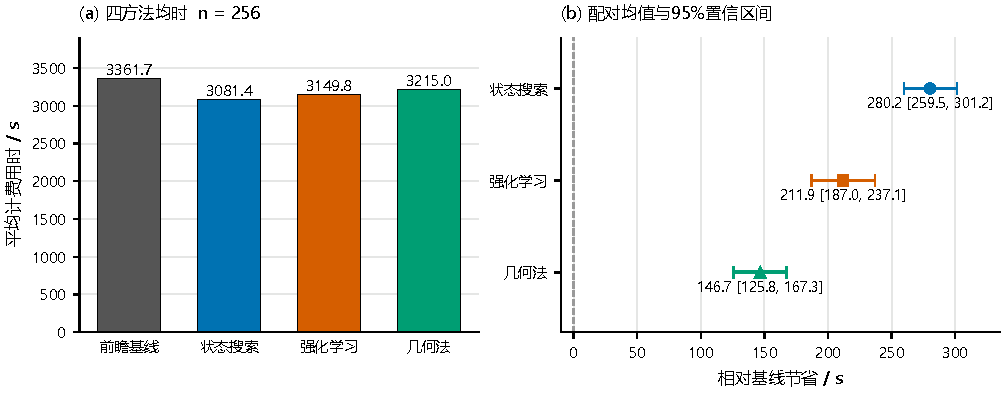
\includegraphics[width=\linewidth,height=\textheight,keepaspectratio,alt={图3 首版四方法在同一256随机场景上的均时与配对节省。右图为相对前瞻基线的95\%配对bootstrap区间，不能当作左图各均时的区间。}]{q23_figures/fig03_comparison.pdf}
\caption{图3 首版四方法在同一256随机场景上的均时与配对节省。右图为相对前瞻基线的95\%配对bootstrap区间，不能当作左图各均时的区间。}
\end{figure}

\begin{figure}[!htbp]
\centering
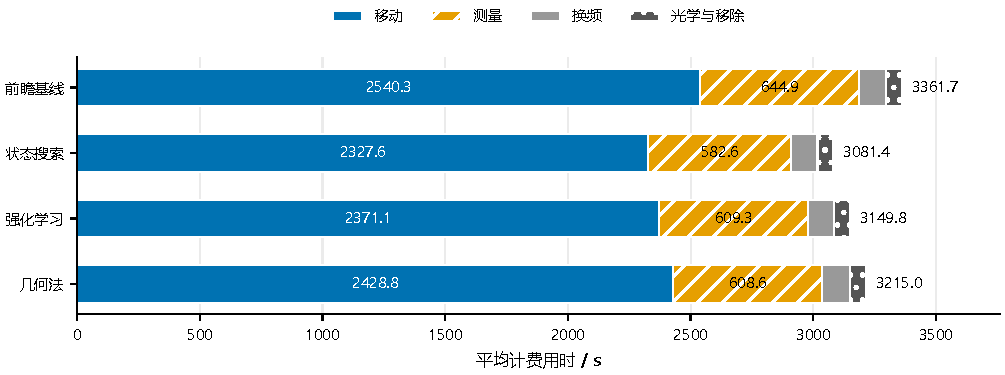
\includegraphics[width=\linewidth,height=\textheight,keepaspectratio,alt={图4 首版随机集的平均费用分解。分项之和等于整局计费用时；移动是主要成本，但扫描与换频的节省同样影响总结果。}]{q23_figures/fig04_costs.pdf}
\caption{图4 首版随机集的平均费用分解。分项之和等于整局计费用时；移动是主要成本，但扫描与换频的节省同样影响总结果。}
\end{figure}

算法计算速度与机器人执行效率需要区分。在同一 Linux CPU 上，四种方案以单线程串行运行已用开发场景，预热后重复两遍，共计每方法 32 局；平均实际计算时间依次为 5.845、0.592、0.170 和 2.098 s/局。PPO 部署计算最快，状态搜索的机器人虚拟耗时最低；该计时包含策略与仿真接口，不等同于纯网络推理延迟，也不是新增的泛化测试。

\subsection{3.10 核心策略的消融分析}\label{ux6838ux5fc3ux7b56ux7565ux7684ux6d88ux878dux5206ux6790}

首先检验可证明无信号的测量能否直接省略。在长轴分位探点策略上，仅增加``候选源区域到待测点的最小距离超过最大接收半径''的删测条件，冻结后 64 局平均从 3132.57 s 降至 3119.32 s，节省 13.25 s，95\% 区间为 {[}9.75,16.97{]} s。移动轨迹保持相同，收益来自检测与换频；未知频道仍执行真实覆盖扫描。这一结果将几何证书的作用与路线调整较清楚地区分开来。

其次，在上述策略基础上仅允许未来覆盖站移到仍满足全场覆盖的位置。另 64 局确认的均时由 3100.20 s 降至 3073.60 s，平均节省 26.59 s，区间为 {[}3.11,53.17{]} s。44 局改善、20 局退化，最坏慢 215.29 s，表明冻结任务上的路线缩短可能被后续发现顺序与定位路径变化抵消。因而，覆盖移站有小幅平均收益证据，但尚不支持所有场景不退化的保证。

后续将真实负反馈与当前候选区域组合，构造更强的相对无信号证书，并加入发现第 16 个源后停止查询未发现频道的规则。在新的 256 局最终随机集上，原 v1 均时为 3122.26 s；仅相对证书、仅数量上限和二者组合分别节省 13.11、1.72 和 14.83 s，对应区间为 {[}11.52,14.74{]}、{[}1.13,2.39{]} 和 {[}13.03,16.70{]} s。组合的改善为 0.475\%，190 胜、66 平、0 负；另 28 局压力集也全部完成。组合在随机集共省 631 次查询，实际节省 3796 s，其中检测 3155 s、换频 641 s，移动费用逐局一致。四局因当前频道改变出现站内重排，故不能笼统声称全部轨迹仅做删除。这批结果支持小幅、可解释的改进，不能与前述不同场景上的均值相减或机械叠加各模块收益。

\begin{figure}[!htbp]
\centering
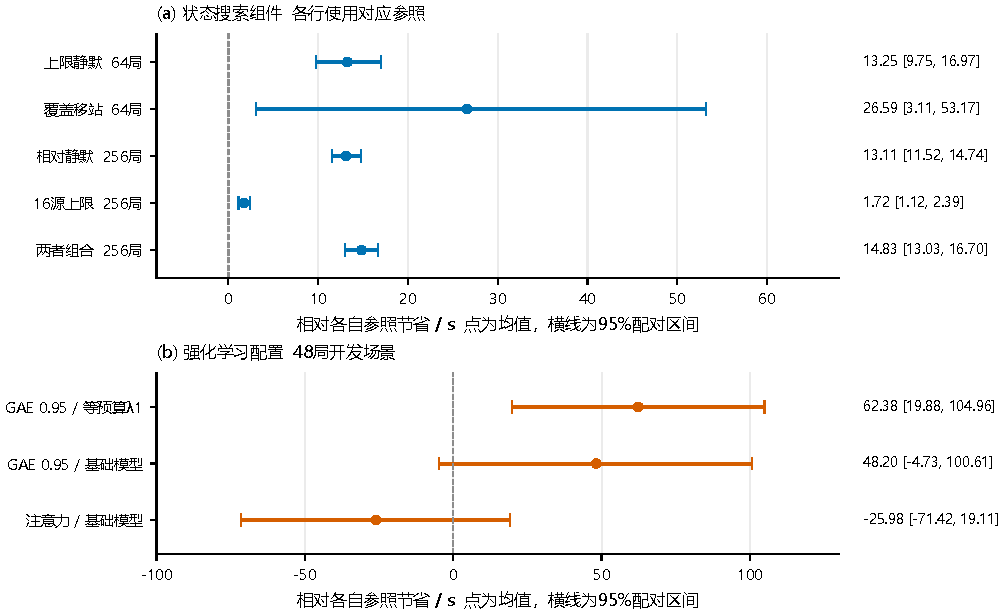
\includegraphics[width=\linewidth,height=\textheight,keepaspectratio,alt={图5 核心组件及训练配置的消融结果。正值表示节省，各行以各自冻结参照计算；上部的64局和256局来自不同实验批次，下部为48局开发结果。不同批次收益不作相加。}]{q23_figures/fig05_ablations.pdf}
\caption{图5 核心组件及训练配置的消融结果。正值表示节省，各行以各自冻结参照计算；上部的64局和256局来自不同实验批次，下部为48局开发结果。不同批次收益不作相加。}
\end{figure}

\subsection{3.11 强化学习的训练与探索结果}\label{ux5f3aux5316ux5b66ux4e60ux7684ux8badux7ec3ux4e0eux63a2ux7d22ux7ed3ux679c}

首版选定的 PPO 模型包含 62882 个参数，以 60 维候选特征和 12 维全局上下文输入策略与价值网络。选定模型在四个训练阶段依次采样 16384、12288、12288、16384 条训练轨迹，合计 57344 条；四阶段均未使用行为克隆。另有18项训练试验、53次开发评估用于比较候选配置，其总采样量与选定模型的训练量分别记录。

在相同基础模型、训练种子和新增 16384 条轨迹下，GAE λ=0.95 模型相较 λ=1 控制组节省 62.38 s，区间为 {[}19.88,104.96{]} s；相较未追加训练的基础模型则节省 48.20 s，区间为 {[}−4.73,100.61{]} s，仍跨零。该对照同时改变优势估计与价值网络的 λ-return 目标，反映这一训练配置的综合影响。强注意力模型相较基础模型反而平均多用 25.98 s，扩展长轴探点后的追加训练、加入覆盖负债特征也未形成稳定收益。它们属于开发集上的机制探索，说明更大的网络、更多动作候选和更久训练并不自动带来改善；尚不能由此判定这些方法族无效。

后续纯 CPU 训练扩大了并行采样，批量也由 32 增为 128，并从同一基础模型进行不同种子的继续训练。因此，现有记录不能将变化单独归因于``从 8 核增加到更多 CPU 核''；核心数、采样预算、更新批量和优化过程同时变化，且逻辑 CPU 槽不等于物理核心。

将后续继续训练模型记为RL-2，已确认的状态搜索尾段精化版记为SS-2，并在同机、同引擎、同48个开发场景配对，RL 均时为 3110.20 s，SS-2为 3101.98 s。RL 平均慢 8.22 s，按``状态用时减 RL 用时''计算的区间为 {[}−58.87,41.21{]} s，尚不能判断平均性能具有可靠差异。RL 每局移动省 29.86 s，但测量多 7.75 次、耗时多 38.75 s，抵消路线收益。该结果与首版独立测试属于不同模型、不同场景；它提示进一步优化应关注信息获取与行程的联合代价，现有结果尚不足以判定两个方法族的最终优劣。

\subsection{3.12 学习行为与官方演练验证}\label{ux5b66ux4e60ux884cux4e3aux4e0eux5b98ux65b9ux6f14ux7ec3ux9a8cux8bc1}

后期RL-2的48条既有轨迹中，48/48 局均先在原点连续测量全部 20 个频道。该模型所属的自由扫描版本已取消初始全扫硬规则，每次可选择覆盖点---频道对，出现正反馈后还可选择定位、清除或中断扫描；因此，这一行为确由已训练策略选择。不过，七个覆盖点、几何候选和可靠退出机制仍是预设的。该现象支持在当前分布和候选空间内采用原点集中扫描的经验合理性，不能证明七点布局或状态压缩全局最优。更早版本的原点扫描由程序固定，因此本项行为分析仅采用解除限制后的模型轨迹。

最后，以冻结的相对无信号组合版进行的既有 50 局官方演练均已完成，全清 657 个源；本批预定跑满50局。平均整局计费用时 2976.87 s，总时间除总源数为 226.55 s/源。这批数据可作为真实接口兼容性与执行效果的补充，但未让各方案在同一官方场景配对，不能据此声称优于 RL 或将其均时与合成测试直接排名。本文统一报告可直接核验的实际耗时；各历史报告的下界口径在辅助证据索引中保留，不用于跨批次排名。

\subsection{3.13 同场景轨迹与退化机制}\label{ux540cux573aux666fux8f68ux8ff9ux4e0eux9000ux5316ux673aux5236}

为了将费用差异对应到具体行动，图6选取首版基线用时最接近256局中位数的场景800035；选择仅依据基线，不依据其他方法的输赢。四种方法使用相同的源位置、接收半径与噪声场，全部清除11个源。在此例中PPO用时2943.02 s，短于状态搜索的3118.22 s，与总体均值的排序不同。这说明代表性轨迹用于解释行为差异，不能替代全部场景上的统计判断。

状态搜索和PPO采用了不同的清除顺序与测点。PPO在该例移动耗时2205.02 s、测量116次；状态搜索移动耗时2311.22 s、测量127次。两项费用均有降低，因而共同解释本例PPO的优势。轨迹中的源坐标只在策略终止后用于展示，规划时不使用这些真值。

\begin{figure}[!htbp]
\centering
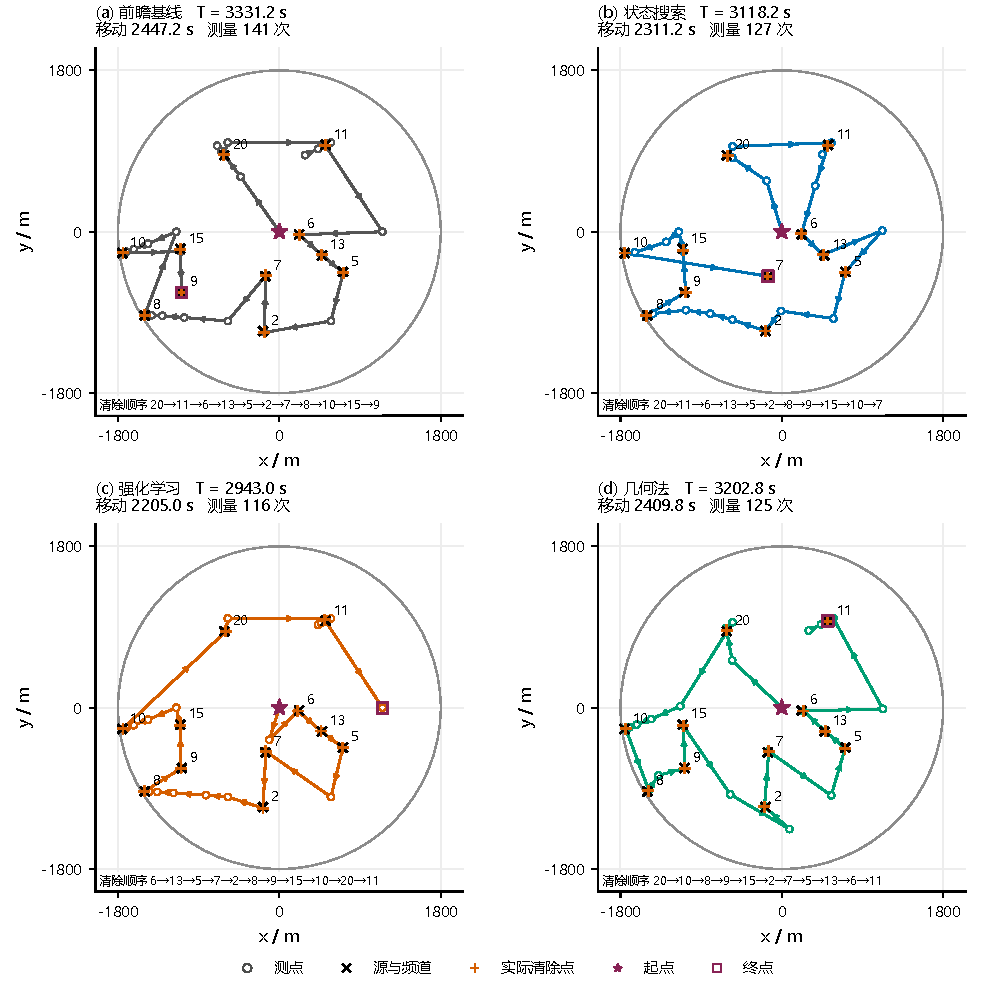
\includegraphics[width=\linewidth,height=\textheight,keepaspectratio,alt={图6 基线中位耗时附近场景800035的四方法真实轨迹。统一坐标比例，箭头表示移动方向，源旁数字为频道，面板底部列出实际清除顺序。同坐标多次测量合并显示位置，但测量次数保留原始计数。}]{q23_figures/fig06_trajectory_median.pdf}
\caption{图6 基线中位耗时附近场景800035的四方法真实轨迹。统一坐标比例，箭头表示移动方向，源旁数字为频道，面板底部列出实际清除顺序。同坐标多次测量合并显示位置，但测量次数保留原始计数。}
\end{figure}

为展示方法的边界，附录还给出各方法相对基线退化最大的案例。状态搜索在800015场景中增加152.08 s移动费用，虽少用25 s测量和2 s换频，最终仍多用125.08 s；PPO在800081场景中多用340.45 s移动、20 s测量和5 s换频，最终多用365.45 s。这些事后选择的反例揭示了长距离折返的代价，不用于估计其总体发生频率，也不据此声称已经识别出网络内部决策的因果原因。

\subsection{3.14 结果讨论与适用范围}\label{ux7ed3ux679cux8ba8ux8bbaux4e0eux9002ux7528ux8303ux56f4}

现有结果支持在本题静止、全向、有限频道且存在可靠几何约束的条件下，以结构化规划作为有效主方案。状态压缩合并当前任务访问顺序，主动定位控制单源信息成本，静默证书删去可证明冗余的查询，覆盖约束负责完整发现。主实验中这一组合取得较低平均任务用时；后期PPO接近状态搜索，则表明学习调度仍具有竞争力。

这种优势不能归结为``固定点可以普遍代替强化学习''。主状态搜索已允许连续移动覆盖站，PPO也依赖人工候选；二者同时利用了题目结构。更大的状态表示、更充分的训练、不同源分布或移动源环境仍可能改变结论。有限任务模型的最优性、连续在线策略的最优性和官方演练的成功记录属于不同层次，本稿只在各自证据范围内提出判断。

\FloatBarrier
\section{参考文献}\label{ux53c2ux8003ux6587ux732e}

{[}1{]} Held M, Karp R M. A Dynamic Programming Approach to Sequencing Problems. Journal of the Society for Industrial and Applied Mathematics, 1962, 10(1):196--210. doi:10.1137/0110015.

{[}2{]} Hart P E, Nilsson N J, Raphael B. A Formal Basis for the Heuristic Determination of Minimum Cost Paths. IEEE Transactions on Systems Science and Cybernetics, 1968, 4(2):100--107. doi:10.1109/TSSC.1968.300136.

{[}3{]} Schulman J, Wolski F, Dhariwal P, et al.~Proximal Policy Optimization Algorithms. arXiv:1707.06347, 2017.

{[}4{]} Schulman J, Moritz P, Levine S, et al.~High-Dimensional Continuous Control Using Generalized Advantage Estimation. International Conference on Learning Representations, 2016.

{[}5{]} Agarwal R, Schwarzer M, Castro P S, et al.~Deep Reinforcement Learning at the Edge of the Statistical Precipice. Advances in Neural Information Processing Systems, 2021, 34:29304--29320.

\clearpage
\section{附录A 实验来源与复核口径}\label{ux9644ux5f55a-ux5b9eux9a8cux6765ux6e90ux4e0eux590dux6838ux53e3ux5f84}

各批次的代码、权重身份与来源SHA256见辅助材料 结构化实验证据索引。下表仅用于定位证据，原始研究目录保留完整动作记录；本轮论文整理未重新运行策略或训练模型。

\Needspace{38mm}
\begin{center}\small 表4 已有实验的来源和用途\end{center}
\nopagebreak
\begin{longtable}[]{@{}lll@{}}

\toprule\noalign{}
证据 & 实验批次与样本 & 用途与边界 \\
\midrule\noalign{}
\endfirsthead
\toprule\noalign{}
证据 & 实验批次与样本 & 用途与边界 \\
\midrule\noalign{}
\endhead
\bottomrule\noalign{}
\endlastfoot
E01至E03 & 首版256随机与28压力 & 四方法完整方案对比，分布分开 \\
E04 & 每方法32局串行计时 & 已用开发场景上的计算开销 \\
E05、E06 & 各64局冻结后确认 & 上限静默、覆盖移站单组件增益 \\
E07 & 新256随机及28压力 & 相对静默、16源上限及组合 \\
E08至E10 & 训练链及开发端点 & PPO预算、GAE与失败探索 \\
E11、E12 & 后期48开发场景 & RL配对结果与原点全扫诊断 \\
E13 & 既有50局官方演练 & 冻结组合版的接口与执行验证 \\
\end{longtable}

图1、图2为解析或算法示意；图3至图8来源于既有数值记录。图6按基线中位耗时选取，图7和图8为事后最大退化例，不混入新增独立测试结论。上述随机评估沿用其原始冻结与数据分割记录；不将已经用于开发的场景重新称为未见测试。

写作组织参考了官方公开的2018年国赛B217与A440两篇匿名展示论文，其出处与获奖展示依据保存在 \texttt{references/references.md}。它们只作为表达范例，本题公式和成绩均以本项目实现及实验为依据。绘图使用Matplotlib及Scientific Visualization skill，其版本、软件文献和导出清单见配套README与参考资料。

\clearpage
\section{附录B 退化案例的轨迹对照}\label{ux9644ux5f55b-ux9000ux5316ux6848ux4f8bux7684ux8f68ux8ff9ux5bf9ux7167}

图7为状态搜索相对前瞻基线退化最大的首版随机场景。图8为PPO相对前瞻基线退化最大的场景。两图均显示全部四方法，不因展示负例而省略其他方法结果。

\begin{figure}[!htbp]
\centering
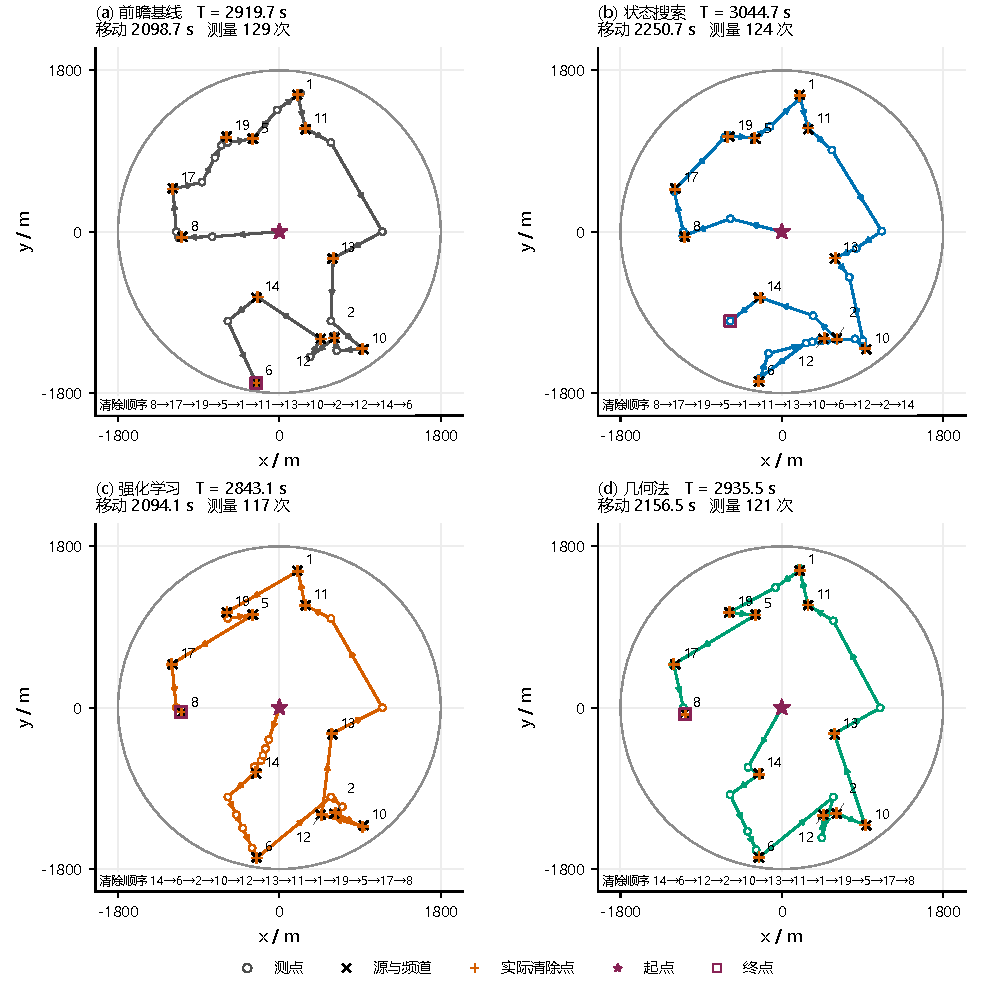
\includegraphics[width=\linewidth,height=\textheight,keepaspectratio,alt={图7 状态搜索最大退化场景800015。状态搜索虽减少检测，却因移动增长而较基线慢125.08 s；此例为事后诊断选择。}]{q23_figures/fig07_trajectory_state_worst.pdf}
\caption{图7 状态搜索最大退化场景800015。状态搜索虽减少检测，却因移动增长而较基线慢125.08 s；此例为事后诊断选择。}
\end{figure}

\begin{figure}[!htbp]
\centering
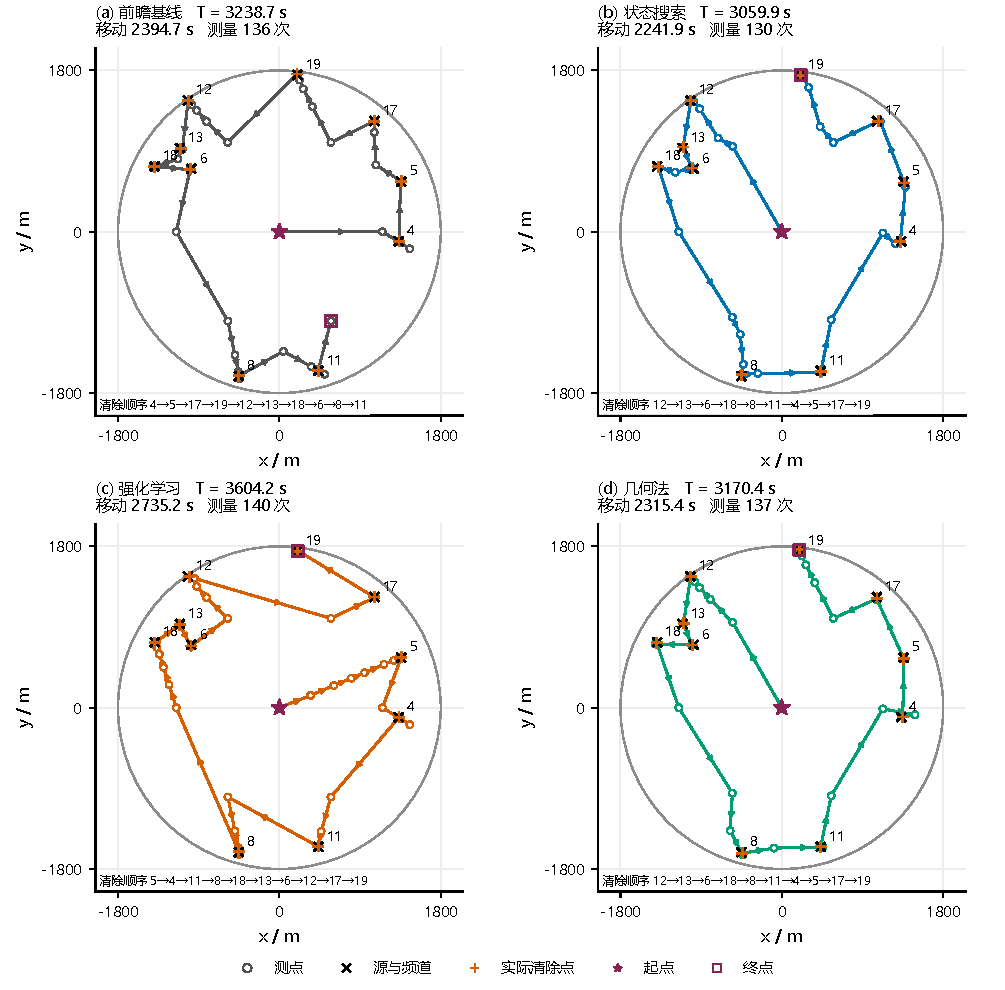
\includegraphics[width=\linewidth,height=\textheight,keepaspectratio,alt={图8 PPO最大退化场景800081。该例主要额外代价来自移动，PPO较基线慢365.45 s；此例不表示总体发生频率。}]{q23_figures/fig08_trajectory_rl_worst.pdf}
\caption{图8 PPO最大退化场景800081。该例主要额外代价来自移动，PPO较基线慢365.45 s；此例不表示总体发生频率。}
\end{figure}

\FloatBarrier
